% LTeX: language=it

\documentclass{../.common/high-school-notebook}

\hypersetup{
  pdftitle={Quaderno delle regole - Fisica},
  pdfauthor={Tommaso Bocchietti},
  pdfsubject={High School Notebook},
}

\begin{document}

\title{Quaderno delle regole - Fisica}
\author{Tommaso Bocchietti}

\maketitle

\begin{figure}[H]
    \centering
    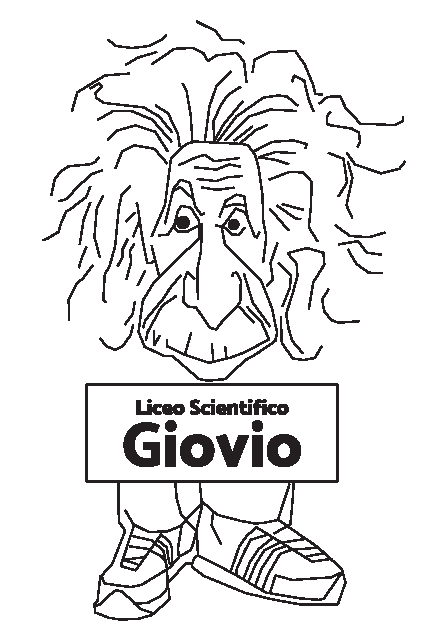
\includegraphics[width=0.7\textwidth]{../.common/Einstein_Logo}
    \label{fig:Einstein_Logo}
\end{figure}


\clearpage
\tableofcontents

% \clearpage
% % LTeX: language=it

\section{Basi della fisica}


% \clearpage
% % LTeX: language=it

\section{I moti}

% % LTeX: language=it

\section{Leggi di Newton}

% % LTeX: language=it

\section{Lavoro}


% \clearpage
% % LTeX: language=it

\section{I moti del piano}

% % LTeX: language=it

\section{Il modello standard}

% % LTeX: language=it

\section{Forza gravitazionale}

% % LTeX: language=it

\section{Quantità di moto e Momento angolare}

% % LTeX: language=it

\section{Termologia}

% % LTeX: language=it

\section{Legge dei gas}

% % LTeX: language=it

\section{Termodinamica}

% % LTeX: language=it

\section{Entropia}


\clearpage
% % LTeX: language=it

\section{Moto armonico}

% % LTeX: language=it

\section{Le onde}

% % LTeX: language=it

\section{Suono}

% % LTeX: language=it

\section{Ottica}

% % LTeX: language=it

\section{Elettrostatica}

L'elettrostatica studia le cariche elettriche stazionarie nel tempo.
Gli elettroni hanno massa $m_e = \SI{9.109e-31}{\kilo\gram}$ e carica negativa.
I protoni hanno massa $m_p = \SI{1.673e-27}{\kilo\gram}$ e carica positiva.
La carica elementare equivale a $e = \SI{1.602e-19}{\coulomb}$.

Un corpo si dice isolante se i suoi elettroni sono dissi e impossibilitati a muoversi, ma solo direzionarsi.
É un conduttore se gli elettroni sono liberi di muoversi e spostarsi.

\subsection{Legge di Coulomb}

Per il calcolo della forza tra due cariche puntiformi si usa la legge di Coulomb:

\begin{equation*}
    F = k_0 \frac{Q_1 Q_2}{r^2}
\end{equation*}

Dove $k_0 = \frac{1}{4\pi\varepsilon_0}$, con $\varepsilon_0 = \text{Costante dielettrica del vuoto} = \SI{8.854e-12}{\coulomb\squared\per\newton\per\meter\squared}$.

I materiali si possono caricare per strofinio, contatto o induzione. Gli isolanti, o dielettrici, si possono solo polarizzare (polarizzazione).

Costante dielettrica relativa $\varepsilon = \varepsilon_r \varepsilon_0$.

\subsection{Il campo elettrico}

Un campo vettoriale è una funzione che associa a ogni punto dello spazio, un vettore che specifica in modulo, direzione e verso, una data grandezza vettoriale.

Forza generata da un campo elettrico:

\begin{equation*}
    \vec{F} = q \vec{E} \rightarrow \SI{}{\newton} = \SI{}{\coulomb} \cdot \frac{\SI{}{\newton}}{\SI{}{\coulomb}}
\end{equation*}

Dove $q = \text{carica di prova}$.

Rappresentazione grafica:

% TODO: carica elettrica con linee di campo
% TODO: dipolo elettrico con linee di campo

\subsection{Flusso del campo elettrico / Teorema di Gauss}

\begin{align*}
    \text{Per superfici aperte}: & \Phi_S(\vec{E}) = \int_S \vec{E} \cdot \vec{S} \, dS = \sum_{i = 1}^{N} \vec{E_i} \cdot \vec{\Delta S_i}            \\
    \text{Per superfici chiuse}: & \Phi_\Omega(\vec{E}) = \frac{Q_{tot}}{\varepsilon}, \text{con } Q_{tot} = \text{carica totale contenuta in } \Omega
\end{align*}

% TODO: esempio di superficie aperta
% TODO: esempio di superficie chiusa con carica interna

\subsection{Forme di campo elettrico in casi noti}

Ipotizzando di essere nel vuoto, e quindi di avere $\varepsilon = \varepsilon_0$, possiamo dare la definizione di $\vec{E}$ per alcuni casi particolari.

\begin{itemize}
    \item Carica puntiforme: $\vec{E} = k_0 \frac{Q}{r^2} \hat{r}$
    \item Piano infinito uniformemente carico: $\vec{E} = \frac{\sigma}{2\varepsilon_0} \hat{n}$, con $\sigma = \text{densità di carica superficiale} \SI{}{\coulomb\per\meter\squared}$
    \item Filo infinito uniformemente carico: $\vec{E} = \frac{\lambda}{2\pi\varepsilon_0 r} \hat{r}$, con $\lambda = \text{densità di carica lineare} \SI{}{\coulomb\per\meter}$ e $r = \text{distanza dal filo}$
    \item Una sfera, al suo esterno: $\vec{E} = k_0 \frac{Q}{r^2} \hat{r}$ (essenzialmente una carica puntiforme)
    \item Una sfera conduttrice, al suo interno: $\vec{E} = 0$ perché le cariche si distribuiscono sulla superficie
    \item Una sfera dielettrica, al suo interno: $\vec{E} = r \cdot k_0 \frac{Q}{R^3} \hat{r}$, con $Q = \text{carica compresa nel volume di raggio} r$
    \item In un condensatore piano: $\vec{E} = \frac{\sigma}{\varepsilon_0}$. All'esterno delle barriere, $\vec{E} = 0$
\end{itemize}

\subsection{Energia potenziale elettrica}

L'energia potenziale elettrica tra due cariche puntiformi è:

\begin{equation*}
    U = k_0 \frac{Q_1 Q_2}{r}
\end{equation*}

% TODO: grafico dell'energia potenziale elettrica caso >0 e caso <0

In generale: $U = L = \vec{F} \cdot \vec{s} = q \vec{E} \cdot \text{distanza dalla fonte di campo}$

\subsection{Potenziale elettrico}

Il potenziale elettrico è una funzione scalare che associa a ogni punto dello spazio un valore scalare che specifica l'energia potenziale elettrica di una carica di prova $q$ in quel punto.

\begin{equation*}
    V = \frac{U}{q} = \frac{L}{q} = \frac{\vec{F} \cdot \vec{s}}{q} = \vec{E} \cdot \vec{s}
\end{equation*}

In generale, definito $\Delta V = V_B - V_A$ differenza di potenziale, si ha:

\begin{equation*}
    \Delta V = -\vec{E} \cdot \Delta \vec{s} \rightarrow L = U_A - U_B = - q \Delta V
\end{equation*}

Partendo quindi da $U_{A \rightarrow B} = -q \Delta V = -q (V_B - V_A)$, abbiamo che il lavoro è positivo, e quindi le cariche si spostano autonomamente, se la carica $q$ è:

\begin{itemize}
    \item Positiva, e allora passa da potenziale maggiore a potenziale minore $\rightarrow$ $V_A > V_B$
    \item Negativa, e allora passa da potenziale minore a potenziale maggiore $\rightarrow$ $V_A < V_B$
\end{itemize}

% TODO: schemino di una carica immersa in un campo elettrico con valutazioni su V U e L

Una superficie equipotenziale è il luogo dei punti dello spazio aventi lo stesso potenziale elettrico.

Un esempio è il condensatore piano, che forma tra le sue armature una serie di superfici equipotenziali.

\begin{figure}[H]
    \centering
    \begin{tikzpicture}

        % Draw walls
        \draw[line width=2mm] (0,0) -- (0,3);
        \draw[line width=2mm] (5,0) -- (5,3);

        % Draw electric field lines
        \foreach \y in {0.5,1.5,2.5}
        \draw[postaction={
                    decorate,
                    decoration={
                            markings,
                            mark=between positions 0.2 and 1 step 1.5cm with {\arrow{latex}}
                        }}] (0,\y) -- (4.9,\y);

        % Draw equipotential lines
        \foreach \x in {1.5,3.5}
        \draw[dashed, color=red] (\x, 0) -- (\x,3);

        % Draw equipotential lines
        \foreach \y in {0.5,1,...,2.5}
            {
                \node at (-0.5,\y) {+};
                \node at ( 5.5,\y) {-};
            }
    \end{tikzpicture}
    \caption{Condensatore piano con \textcolor{red}{superfici equipotenziali}}
\end{figure}

\subsection{Circuitazione del campo elettrico lungo una linea chiusa orientata}

É una legge che serve per dimostrare che il campo elettrico $\vec{E}$, rimane costante ed è quindi conservativo.

\begin{equation*}
    \oint_\mathcal{L} \vec{E} = \sum_{i = 1}^{n} \vec{E} \cdot \vec{\Delta s_i}
\end{equation*}

Visto che il campo elettrico è conservativo, deve valere che $\oint_\mathcal{L} \vec{E} = 0$ sempre, ammesso che la linea $\mathcal{L}$ sia chiusa.

\subsection{Distribuzione delle cariche nei conduttori}

Le cariche tendono sempre a mettersi sulle superfici esterne.
L'interno dunque di un conduttore rimane con $\vec{E} = 0$, e $V_{interna} = V_{superficie}$ e dunque $\Delta V = 0$.

Il potere delle punte è un fenomeno correlato alla distribuzione delle cariche sui conduttori per cui si ha $S_{punta} \approx 0$ e quindi $\vec{E} = \frac{Q}{S\varepsilon} = \infty$.
Da questo ne deriva che alcuni cariche possono essere espulse dal conduttore generando così un vento elettrico.

\subsection{Teorema di Coulomb}

Per calcolare il campo elettrico sulla superficie di un conduttore si ha $\vec{E} = \frac{\sigma}{\varepsilon}$

% TODO: disegno conduttore con superficie elettrizzata

\subsection{Capacità di un condensatore}

É definita come il rapporto tra la carica elettrica e il potenziale elettrico:

\begin{equation*}
    C = \frac{Q}{V} \SI{}{\farad} = \SI{}{\coulomb\per\volt}
\end{equation*}

Corrisponde alla quantità di carica che può contenere un conduttore.

\begin{itemize}
    \item Per una sfera conduttrice: $C = 4\pi\varepsilon_0 R$
    \item Per un condensatore piano: $C = \varepsilon_0 \frac{S}{d}$, con $S = \text{superficie delle armature}$ e $d = \text{distanza tra le armature}$
\end{itemize}

\subsection{Energia immagazzinata in un condensatore}

Corrisponde al lavoro compiuto per caricare il condensatore

\begin{equation*}
    W_c = \frac{1}{2} \frac{Q^2}{C} = \frac{1}{2} C V \SI{}{\joule}
\end{equation*}

\subsection{Densità di energia in un condensatore}

É il rapporto tra l'energia immagazzinata e il volume del condensatore tra le pareti.

\begin{equation*}
    w_{\vec{E}} = \frac{W_c}{Sd} = \frac{1}{2} \varepsilon_0 E^2 \SI{}{\joule\per\meter\cubed}
\end{equation*}

\subsection{Proprietà fondamentali del campo elettrico}

Si riportano qui le due proprietà fondamentali del campo elettrico:

\begin{itemize}
    \item Flusso del campo elettrico da una superficie chiusa: $\Phi_\Omega(\vec{E}) = \frac{Q_{tot}}{\varepsilon}$
    \item Circuitazione del campo elettrico lungo una linea chiusa orientata: $\oint_\mathcal{L} \vec{E} = 0$
\end{itemize}























% % LTeX: language=it

\section{Corrente elettrica}


\clearpage
% % LTeX: language=it

\section{Campo magnetico}

% % LTeX: language=it

\section{Corrente indotta}

% LTeX: language=it

\section{Induttanza}

% % LTeX: language=it

\section{Corrente alternata}

% % LTeX: language=it

\section{Equazioni di Maxwell}

Nel 1865, Maxwell comprese che il campo elettrico e il campo magnetico si influenzavano reciprocamente.
Egli propose delle equazioni basate sul flusso e sulla circuitazione di $\vec{E}$ e $\vec{B}$ per dimostrarlo.

\subsection{Circuitazione di $\vec{E}$ lungo $\mathcal{L}$}

Partendo da $\oint_{\mathcal{L}} \vec{E} = 0$, Maxwell dimostrò che tale circuitazione è legata alla forza elettromotrice $\text{fem}(\vec{B})$ attraverso:

\begin{equation*}
    \oint_{\mathcal{L}} \vec{E} = - \frac{\Delta \Phi_S(\vec{B})}{\Delta t}
\end{equation*}

Questo indica che un campo elettrico può essere generato da cariche elettriche o da campi magnetici variabili nel tempo.

\subsection{Circuitazione di $\vec{B}$ lungo $\mathcal{L}$}

Partendo da $\oint_{\mathcal{L}} \vec{B} = \mu_0 \cdot I_{\text{concatenata}}$, Maxwell introdusse la corrente di spostamento $I_s = \varepsilon_0 \cdot \frac{\Delta \Phi_S(\vec{E})}{\Delta t}$.
Quindi, la circuitazione diventa:

\begin{equation*}
    \oint_{\mathcal{L}} \vec{B} = \mu_0 \cdot \left( I_c + I_s \right) = \mu_0 \cdot \left( I_c + \varepsilon_0 \cdot \frac{\Delta \Phi_S(\vec{E})}{\Delta t} \right)
\end{equation*}

Questo dimostra che un campo magnetico può essere generato da correnti elettriche o da campi elettrici variabili nel tempo.

\subsection{Definizione di campo elettromagnetico}

La combinazione delle equazioni di Maxwell porta alla definizione del campo elettromagnetico, in cui $\vec{E}$ e $\vec{B}$ si influenzano reciprocamente senza la necessità di un mezzo materiale.

\begin{align*}
    \Phi_\Omega(\vec{E})        & = \frac{Q_{\text{tot}}}{\varepsilon}                                                           \\
    \Phi_\Omega(\vec{B})        & = 0                                                                                            \\
    \oint_{\mathcal{L}} \vec{E} & = - \frac{\Delta \Phi_S(\vec{B})}{\Delta t}                                                    \\
    \oint_{\mathcal{L}} \vec{B} & = \mu_0 \cdot \left( I_c + \varepsilon_0 \cdot \frac{\Delta \Phi_S(\vec{E})}{\Delta t} \right)
\end{align*}

La risoluzione di queste equazioni conduce alla definizione delle onde elettromagnetiche, come ad esempio la luce.

% % LTeX: language=it

\section{Onde elettromagnetiche}

Le onde elettromagnetiche sono il risultato della propagazione simultanea di un campo magnetico $\vec{B}$ e di un campo elettrico $\vec{E}$, perpendicolari tra loro.
Il primo a provare a l'esistenza di queste onde fu il fisico Hertz, che provocando una scintilla, riuscì a produrne un altra in due punti diversi della stanza.
La prima scintilla aveva prodotto un onda elettromagnetica.

\begin{figure}[H]
    \centering

    % https://tikz.net/electromagnetic_wave/
    % Electromagnetic wave - colored
    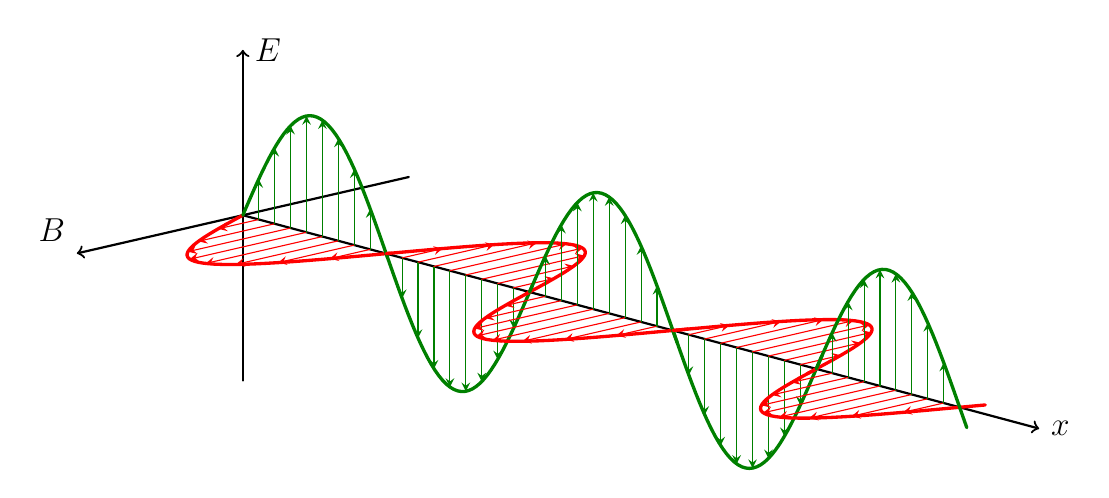
\begin{tikzpicture}[x=(-15:1.2), y=(90:1.0), z=(-150:1.0),
            line cap=round, line join=round,
            axis/.style={black, thick,->},
            vector/.style={>=stealth,->}]
        \large
        \def\A{1.5}
        \def\nNodes{5} % use even number
        \def\nVectorsPerNode{8}
        \def\N{\nNodes*40}
        \def\xmax{\nNodes*pi/2*1.01}
        \pgfmathsetmacro\nVectors{(\nVectorsPerNode+1)*\nNodes}

        \def\drawENode{ % draw E node and vectors with some offset
            \draw[Green,very thick,variable=\t,domain=\iOffset*pi/2:(\iOffset+1)*pi/2*1.01,samples=40]
            plot (\t,{\A*sin(\t*360/pi)},0);
            \foreach \k [evaluate={\t=\k*pi/2/(\nVectorsPerNode+1);
                        \angle=\k*90/(\nVectorsPerNode+1);}]
            in {1,...,\nVectorsPerNode}{
                    \draw[vector,Green]  (\iOffset*pi/2+\t,0,0) -- ++(0,{\A*sin(2*\angle+\iOffset*180)},0);
                }
        }
        \def\drawBNode{ % draw B node and vectors with some offset
            \draw[Red,very thick,variable=\t,domain=\iOffset*pi/2:(\iOffset+1)*pi/2*1.01,samples=40]
            plot (\t,0,{\A*sin(\t*360/pi)});
            \foreach \k [evaluate={\t=\k*pi/2/(\nVectorsPerNode+1);
                        \angle=\k*90/(\nVectorsPerNode+1);}]
            in {1,...,\nVectorsPerNode}{
                    \draw[vector,Red]  (\iOffset*pi/2+\t,0,0) -- ++(0,0,{\A*sin(2*\angle+\iOffset*180)});
                }
        }

        % MAIN AXES
        \draw[axis] (0,0,0) -- ++(\xmax*1.1,0,0) node[right] {$x$};
        \draw[axis] (0,-\A*1.4,0) -- (0,\A*1.4,0) node[right] {$E$};
        \draw[axis] (0,0,-\A*1.4) -- (0,0,\A*1.4) node[above left] {$B$};

        % draw (anti-)nodes
        \foreach \iNode [evaluate={\iOffset=\iNode-1;}] in {1,...,\nNodes}{
                \ifodd\iNode \drawBNode \drawENode % E overlaps B
                \else        \drawENode \drawBNode % B overlaps E
                \fi
            }

    \end{tikzpicture}
    \caption{Onda elettromagnetica}
\end{figure}

\subsection{Velocità dell'onda}

La velocità dell'onda elettromagnetica è determinata da $v = \frac{1}{\sqrt{\mu \varepsilon}}$, che nel vuoto diventa $v = c = 3 \cdot 10^8 \frac{m}{s}$.

L'indice di rifrazione del mezzo, $n$, è legato a $\sqrt{\mu_r \varepsilon_r}$.

\subsection{Onde elettromagnetiche piane}

Considerando un'antenna che genera onde sferiche a distanze significative, queste possono essere approssimate come onde piane. Le onde elettromagnetiche sono trasversali, con $\vec{E} \perp \vec{B}$ e $E = c \cdot B$ nel vuoto, indicando che $E \gg B$.

\subsection{Energia e quantità di moto}

Le onde elettromagnetiche trasportano energia e quantità di moto. Le forme di energia massime ($w_{E,B}$) e medie ($\overline{w_{E,B}}$) sono date da:

\begin{align*}
    w_E            & = \frac{1}{4} \varepsilon_0 E_0^2 \\
    w_B            & = \frac{1}{4 \mu_0} B_0^2         \\
    \overline{w_E} & = \frac{1}{2} \varepsilon_0 E^2   \\
    \overline{w_B} & = \frac{1}{2 \mu_0} B^2
\end{align*}

La densità volumica di energia è data da $\overline{w} = \overline{w_E} + \overline{w_B}$. L'energia totale nello spazio è $\mathcal{E} = A c \Delta t \overline{w}$.

L'irradiamento $I = \frac{P}{A}$ implica $E_r = \frac{\mathcal{E}}{A \Delta t} = c \overline{w}$.

\subsection{Quantità di moto e pressione di radiazione}

La quantità di moto, $p$, è legata alla forza ricevuta da un corpo a causa della propagazione dell'onda: $p = \frac{\mathcal{E}}{c}$.

La pressione di radiazione, $P_r$, è definita come $P_r = \frac{E_r}{c}$, associando la forza per unità di area alla propagazione dell'onda.

\subsection{Polarizzazione di onde elettromagnetiche}

Un'onda è polarizzata se $\vec{E}$ e $\vec{B}$ hanno direzioni ben definite nello spazio. La luce non polarizzata è un insieme casuale di onde.

% TODO: Aggiungere grafico campo E polarizzato (vettori apparatenenti allo stesso piano)

Il polarizzatore lineare filtra solo le onde con $\vec{E}$ in una specifica direzione.

% TODO: Aggiungere grafico polarizzatore lineare con spiegazione a fianco inceve che qui sotto

Le linee nere del polarizzatore, costituite da materiale conduttore, bloccano la componente orizzontale dell'onda, consentendo solo la componente verticale.

Se un fascio polarizzato attraversa un filtro inclinato rispetto a $\vec{E}$, la trasmissione è $E_r = E_r^{(0)} \cos^2(\alpha)$, permettendo solo la componente trasversale al filtro.
% % LTeX: language=it

\section{Spettro elettromagnetico}

Lo spettro elettromagnetico è l'insieme delle frequenze delle onde elettromagnetiche.
É possibile suddividere lo spettro elettromagnetico in sette grandi categorie:

\begin{figure}[H]
    \centering
    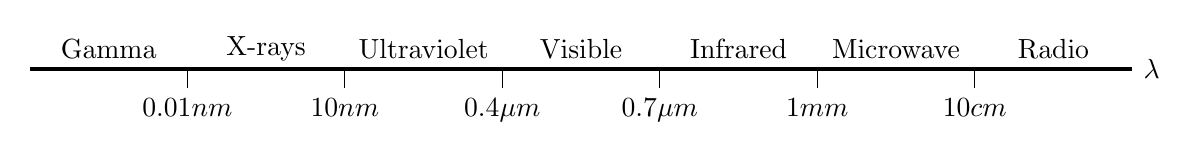
\begin{tikzpicture}[scale=0.5]
        % Spectrum lines
        \draw[ultra thick] (0,0) -> (28,0) node[right] {$\lambda$};

        % Wavelengths
        \foreach \w/\label in {4/$0.01nm$, 8/$10nm$, 12/$0.4\mu m$, 16/$0.7\mu m$, 20/$1mm$, 24/$10cm$}
            {
                \draw (\w,0) -- (\w,-0.5) node[below] {\label};
            }

        % Labels
        \foreach \w/\label in {2/Gamma, 6/X-rays, 10/Ultraviolet, 14/Visible, 18/Infrared, 22/Microwave, 26/Radio}
            {
                \node at (\w, 0.5) {\label};
            }

        % % Rainbow-colored band in the visible region (between 12 and 16)
        % \fill[red] (12,0) rectangle (12.8,0.2);
        % \fill[orange] (12.8,0) rectangle (13.6,0.2);
        % \fill[yellow] (13.6,0) rectangle (14.4,0.2);
        % \fill[green] (14.4,0) rectangle (15.2,0.2);
        % \fill[cyan] (15.2,0) rectangle (16,0.2);

    \end{tikzpicture}
    \caption{Spettro elettromagnetico}
\end{figure}

Conoscendo la lunghezza d'onda, è possibile calcolare la frequenza dell'onda elettromagnetica come $f = \frac{c}{\lambda}$, dove $c$ è la velocità della luce.
Come si può vedere la luce visibile ha $400nm < \lambda < 700nm$, dove $400nm \rightarrow \text{Violato}$ e $700nm \rightarrow \text{Rosso}$.
% % LTeX: language=it

\section{Relatività ristretta}

\subsection{Velocità della luce e sistemi di riferimento}

Il valore $c = 3 \cdot 10^8 \si{\meter\per\second}$ è un valore massimo e assoluto che non dipende dal sistema di riferimento (S.R.) considerato.
Si ricorda che un S.R.I. (inerziale) è un sistema che di muove di moto rettilineo uniforme e quindi senza accelerazioni.
Essendo $c$ un invariante, allora o la meccanica di Newton/Galileo o l'elettromagnetismo sono sbagliate.
La relatività corregge le formule della meccanica classica.

\subsubsection{Esempio di uno shuttle in movimento che spara due raggi laser}

% TODO: disegno dello shuttle con interpretazione classica della velocità (v+c, v-c) e relativistica (c)

\subsection{L'esperimento di Michelson-Morley (1887)}

Aveva lo scopo di dimostrare l'effetto del vento d'etere sulla velocità della luce $c$.

% TODO: disegno del vento d'etere con sole e Terra orbitante

La Terra compiendo un moto di rivoluzione "naviga" in questa sostanza, in $T_1$ contro vento e in $T_2$ a favore.
Quindi secondo Galileo $c_1 < c$ perché influenzato dal vento, e $c_2 > c$ perché velocizzato dall'etere.
Per osservare la velocità, i fisici costruirono un'interferometro costituito da diversi specchi e una lastra semi-argentata che divide il raggio $1$.

% TODO: disegno dell'interferometro

Il raggio $R_1$  si rifrange su $S_{p-s}$ e si divide in $R_2$ e $R_3$.
Uno dei due viaggia controvento o a favore e quindi $\Delta t_2 = \frac{l}{v+c} + \frac{l}{v-c}$ = $\frac{2l}{c} \cdot \frac{1}{1-\frac{v^2}{c^2}}$ e $\Delta t_3 = \frac{2l}{\sqrt{c^2-v^2}} = \frac{2l}{c} \cdot \frac{1}{\sqrt{1-\frac{v^2}{c^2}}}$.

Si ottiene così una ipotetica fase tra i due raggi di:

\begin{equation*}
    \Delta \phi_{ipotesi} = \Delta t_2 - \Delta t_3 = \frac{2l}{c} \cdot \left( \frac{1}{1-\frac{v^2}{c^2}} - \frac{1}{\sqrt{1-\frac{v^2}{c^2}}} \right)
\end{equation*}

Essendo $R_4 = R_2 + R_3$, se c'è una certa fase allora si creeranno dei fronti so'onda su S.
Da questi si ricava il $v$ del vento d'etere.

Risultato negativo: $c$ non varia quindi l'etere on influenzava la luce.

\subsection{Gli assiomi della teoria della relatività ristretta}

\begin{itemize}
    \item Le leggi e i principi della fisica hanno la stessa forma in tutti i sistemi di riferimento inerziali (S.R.I.).
    \item La velocità della luce $c$ nel vuoto è la stessa in tutti i S.R.I., indipendentemente dal moto del sistema o della sorgente da cui la luce è emessa.
\end{itemize}

\subsection{La simultaneità}

Definizione operativa: due eventi $E_1 / E_2$ sono simultanei quando, preso $P_3 = \frac{P_1 + P_2}{2}$, il segnale luminoso emesso da $E_1$ impiega lo stesso $\Delta t_1$ per raggiungere $P_3$ del segnale luminoso emesso da $E_2$, $\Delta t_2 \rightarrow $

% TODO: disegno della simultaneità (omino e segnali acustici)

La simultaneità diventa però relativa se consideriamo più di un solo S.R.I.

\subsubsection{Esempio del treno e dei lampi di luce}

Presi $E_1$ e $E_2$  simultanei per il sistema di riferimento $O_{terra}$, essi non sono più simultanei per il sistema di riferimento $O_{movimento}$.

% TODO: disegno del treno con lampi di luce

\subsection{La dilatazione dei tempi}

Due orologi sono sincronizzati se al tempo $t_0$, l'orologio $1$ lancia un segnale luminoso all'orologio $2$, e questo, quando il raggio lo raggiunge segna $t = t_0 + \frac{d}{c}$

% TODO: disegno degli orologi e della distanza tra i due

Se però abbiamo due S.R.I. in moto relativo, allora il tempo $t$ non scorre più alla stessa velocità tra i due sistemi, ma che nel sistema in movimento il tempo scorre più lentamente rispetto a quello fermo.

\subsubsection{Esempio dei laser in movimento}

% TODO: disegno dei laser in movimento

Dai disegni sopra, si nota come il cammino percorso dal laser cambi in base alla posizione dell'osservatore.
In particolare:

\begin{itemize}
    \item Osservatore a bordo del carrello laser (in movimento): $t = \frac{2d}{c}$
    \item Osservatore fermo: $t' = \frac{2d}{c} \cdot \frac{1}{\sqrt{1-\frac{v^2}{c^2}}}$
\end{itemize}

Si ha quindi che $\Delta t' > \Delta t$ e quindi che il tempo in un S.R.I. in movimento rispetto a un altro scorre più lentamente.

Si definiscono allora:

\begin{align*}
    \Delta t  & = \text{tempo proprio}                                                        \\
    \Delta t' & = \text{tempo improprio}                                                      \\
    \gamma    & = \frac{1}{\sqrt{1-\frac{v^2}{c^2}}} \quad \text{coefficiente di dilatazione} \\
    \beta     & = \frac{v}{c}
\end{align*}

\subsection{La contrazione delle lunghezze}

Come conseguenza della dilatazione dei tempi, vi è anche la contrazione delle lunghezze.
Essendo $\Delta x = v \cdot \Delta t'$ e $\Delta x' = v \cdot \Delta t$, si ha che:

\begin{equation*}
    \Delta x' = \frac{\Delta x}{\gamma} = \Delta x \cdot \sqrt{1-\frac{v^2}{c^2}}
\end{equation*}

Dove $\Delta x$ è la lunghezza propria del segmento e $\Delta x'$ è la lunghezza impropria, ovvero la lunghezza del segmento visto dall'esterno e da fermo.

Abbiamo quindi che $\Delta t' = \gamma \cdot \Delta t$ e $\Delta x' = \frac{\Delta x}{\gamma}$, con $\gamma$ avente la seguente forma:

\begin{figure}[H]
    \centering
    \begin{tikzpicture}

        \begin{axis}[
                axis lines = left,
                xlabel = $v$,
                ylabel = {$\gamma$},
                xmin = 0,
                xmax = 1,
                ymin = 0,
                ymax = 10,
            ]

            % \node at (axis cs:0.5,-0.5) {$c$};

            % Below the red parabola is defined
            \addplot [
                domain=0:1,
                samples=100,
                color=red,
            ]
            {1/sqrt(1-x^2)};
            \addlegendentry{$\gamma = \frac{1}{\sqrt{1-\frac{v^2}{c^2}}}$}

        \end{axis}

    \end{tikzpicture}
\end{figure}

\subsubsection{Esempio del caso del muone}

Il muone è una particella che si forma nella parte alta dell'atmosfera e ha una vita media di $\Delta t = 2.2 \cdot 10^{-6} \si{\second}$.
Data la sua elevata velocità $v = 0.998c$, per valutarne la possibile distanza $\Delta x$ (vista dalla Terra) che può percorrere prima di decadere, si deve utilizzare la correzione relativistica.
Si ha cosi che:

\begin{figure}[H]
    \begin{minipage}[t]{0.45\textwidth}
        \centering
        Meccanica classica
        \begin{equation*}
            \Delta x = v \cdot \Delta t = 0.998c \cdot 2.2 \cdot 10^{-6} \approx 660 \si{\meter}
        \end{equation*}
    \end{minipage}
    \hfill
    \begin{minipage}[t]{0.45\textwidth}
        \centering
        Relatività ristretta
        \begin{align*}
            \gamma    & = \frac{1}{\sqrt{1-\frac{v^2}{c^2}}} = \frac{1}{\sqrt{1-\frac{(0.998c)^2}{c^2}}} = 15                    \\
            \Delta t' & = \gamma \cdot \Delta t = 15 \cdot 2.2 \cdot 10^{-6} \approx 35 \si{\micro\second}                       \\
            \Delta x  & = \gamma \cdot \Delta x' = v \cdot \Delta t' = 0.998c \cdot 35 \cdot 10^{-6} \approx 10 \si{\kilo\meter}
        \end{align*}
    \end{minipage}
\end{figure}

Da notare che con $\Delta x$ abbiamo calcolato la distanza che il muone può percorrere prima di decadere vista da un osservatore fermo (sulla Terra), mentre con $\Delta x'$ abbiamo calcolato la distanza che il muone può percorrere prima di decadere vista da un osservatore in moto insieme al muone.

In altre parole, al muone sembrerà di aver percorso una distanza decisamente minore rispetto a quella calcolata dall'osservatore fermo (contrazione delle lunghezze).
In maniera duale, al muone sembrerà di essere in vita per un tempo decisamente maggiore rispetto a quello calcolato dall'osservatore fermo (dilatazione dei tempi).

In definitiva, si ha dunque che se per il muone la distanza che percorre è solo di $660 \si{\meter}$, dalla terra il muone percorre una distanza di circa $10 \si{\kilo\meter}$.

\subsection{L'invarianza delle lunghezze perpendicolari al moto relativo}

Si sottolinea ora che la contrazione delle lunghezze avviene solo per le lunghezze parallele al moto relativo, ovvero lungo la direzione del moto.
Per le lunghezze perpendicolari al moto, invece, non vi è alcuna contrazione.

\subsubsection{Esempio del treno e del tunnel}

Un esempio classico che prova logicamente l'invarianza delle lunghezze perpendicolari al moto relativo è quello del treno che attraversa un tunnel.
É infatti un assurdo pensare che il passaggio o meno del treno all'ingresso della galleria dipenda dalla velocità del treno stesso.

\subsection{Le trasformazioni di Lorentz}

Sono delle equazioni per ottenere le coordinate spazio-temporali di un punto materiale in un S.R.I. ($S'$), partendo dalle coordinate di un altro S.R.I. ($S$).
Le trasformazioni di Galileo vengono qui sostituite da quelle di Lorentz:

\begin{figure}[H]
    \begin{minipage}[t]{0.45\textwidth}
        \centering
        Galileo
        \begin{align*}
            x' & = x - vt \\
            y' & = y      \\
            z' & = z      \\
            t' & = t
        \end{align*}
        % TODO: disegno delle trasformazioni di Galieleo
    \end{minipage}
    \hfill
    \begin{minipage}[t]{0.45\textwidth}
        \centering
        Lorentz (dirette e inverse)
        \begin{align*}
            x' & = \gamma \cdot (x - vt)                             \\
            y' & = y                                                 \\
            z' & = z                                                 \\
            t' & = \gamma \cdot \left( t - \frac{\beta}{c} x \right)
        \end{align*}
        \begin{align*}
            x & = \gamma \cdot (x' + vt')                             \\
            t & = \gamma \cdot \left( t' + \frac{\beta}{c} x' \right)
        \end{align*}
    \end{minipage}
    % TODO: disegno delle trasformazioni di Lorentz
\end{figure}

Dove ogni grandezza avente l'apice è relativa al S.R.I. $S'$, mentre quelle senza apice sono relative al S.R.I. $S$.

\subsection{L'intervallo invariante}

Se consideriamo uno spostamento nello spazio, esso può essere rappresentato in infiniti piani cartesiani, con stessa origine $O$.

Per entrambe le rappresentazioni avremo $\Delta s^2 = \Delta x^2 + \Delta y^2 = \Delta X^2 + \Delta Y^2$, e quindi si può vedere che nonostante il S.R. considerato, l'intervallo $\Delta s^2$ è una misura invariante.

In fisica, consideriamo la quaterna ordinata $(x, y, z, t)$ con il nome di "Evento".
Avendo quindi due eventi $E_1$ e $E_2$ in un dato S.R., possiamo calcolare l'intervallo invariante come:

\begin{equation*}
    \Delta \sigma^2 = (c\Delta t)^2 - \Delta x^2 - \Delta y^2 - \Delta z^2 = (c\Delta t)^2 - \Delta s^2
\end{equation*}

Dove $\Delta s^2$ è la distanza spaziale tra i due eventi e $\Delta \sigma^2$ è l'intervallo invariante tra i due eventi.

In base al segno di $\Delta \sigma^2$, possiamo classificare gli eventi in:

\begin{itemize}
    \item $\Delta \sigma^2 > 0$: Eventi casualmente connessi. Se $E_1$ lancia un segnale, esso riesce a raggiungere $E_2$. Si può quindi dire che esiste un S.R. dove $\Delta s = 0$ e $\Delta t = \frac{\sqrt{\Delta s^2}}{c}$.
    \item $\Delta \sigma^2 < 0$: Eventi casualmente non connessi. Un segnale lanciato da $E_1$ non può raggiungere $E_2$. Si può quindi dire che esiste un S.R. dove $\Delta s = \sqrt{-\Delta \sigma^2}$.
    \item $\Delta \sigma^2 = 0$: Solo un segnale luminoso a velocità $c$ può collegare i due eventi, ovvero raggiungere $E_2$ partendo da $E_1$.
\end{itemize}

\subsection{Lo spazio-tempo di Minkowski}

Ad ogni Evento, oltre che definirlo tramite le coordinate spaziali (x, y, z), va definito da un quadrivettore spazio-temporale $(x, y, z, t)$, dove quindi alla definizione 3D se ne aggiunge una, diventando una definizione spazio-tempo in 4D.
Gli eventi sono definiti da $\Delta \sigma$.

Il diagramma di Minkowski è la rappresentazione grafica di eventi, e gli assi sono definiti come $ct(x)$ o $ct(y)$ o $ct(z)$, mentre l'evento $E$ è rappresentato come punto $E(x_0, ct_0)$.

% TODO: disegno del diagramma di Minkowski

Se per esempio consideriamo un raggio di luce che parte in $x_0 = -3m$ al tempo $t_0 = 1s$ e viaggia a $v = c$, allora rispetto a un uomo fermo in $x_0 = 0m$, avremo:

\begin{figure}[H]
    \centering
    \begin{tikzpicture}

        \begin{axis}[
                axis lines = left,
                xlabel = $x$,
                ylabel = {$ct$},
                xmin = -5,
                xmax = 5,
                ymin = 0,
                ymax = 5,
            ]

            \coordinate (E0) at (-3,1);
            \coordinate (E) at (0,4);

            \draw[dashed] (E0) -> (E)+(0.1,0.4);
            \draw (E0) node[below, left] {$E_0$};

        \end{axis}
    \end{tikzpicture}
    \caption{Diagramma di Minkowski applicato al caso 1D}
\end{figure}

% TODO: disegno dell'omino e del raggio di luce

Grazie al diagramma di Minkowski è quindi possibile calcolare dove si troverà il fascio dopo una certo tempo $\Delta t$ o un certo spazio $\Delta x$.

\subsection{La composizione relativistica delle velocità}

Così come per le coordinate, anche per le velocità Galileo non è più corretto.
Per calcolare $u'$, ovvero la velocità di $E$ ma rispetto a $S'$, si ha che:

\begin{figure}[H]
    \begin{minipage}[t]{0.45\textwidth}
        \centering
        Galileo
        \begin{equation*}
            u' = u - v
        \end{equation*}
    \end{minipage}
    \hfill
    \begin{minipage}[t]{0.45\textwidth}
        \centering
        Lorentz (dirette e inverse)
        \begin{equation*}
            u' = \frac{u - v}{1 - \frac{uv}{c^2}}
        \end{equation*}
        \begin{equation*}
            u = \frac{u' + v}{1 + \frac{uv}{c^2}}
        \end{equation*}
    \end{minipage}
\end{figure}

\subsubsection{Esempio dell'astronave e della pallottola}

Per comprendere meglio il concetto di composizione relativistica delle velocità, consideriamo il seguente esempio.
Supponiamo di avere un'astronave che viaggia a $u$ e che spara una pallottola a velocità $v$, entrambe misurate da un osservatore fermo sulla Terra.
Per calcolare la velocità della pallottola rispetto all'astronave, avremo che $v' = \frac{v-u}{1-\frac{uv}{c^2}}$ e non più $v' = v-u$ come in meccanica classica.

% TODO: disegno dell'astronave e della pallottola

\subsection{L'equivalenza tra massa ed energia}

Con relatività si associa energia alla massa, infatti $\Delta E = \Delta m \cdot c^2$.
La massa e l'energia prese singolarmente non sono più invarianti, ma ora vale il principio della conservazione massa-energia.

La massa a riposo $m_0$, è la massa caratteristica del corpo quando $v = 0$, mentre la massa relativistica $m$ è la massa del corpo in movimento.

Si ha quindi che $E_0 = m_0 \cdot c^2$ e $E = m \cdot c^2$, con $m = \gamma \cdot m_0$.

\subsection{La dinamica relativistica}

Consideriamo ora corpi in movimento a velocità $v$, possiamo affermare che l'energia totale è $E = \gamma m_0 c^2$, che $K = (\gamma - 1) m_0 c^2$, che $p_r = \gamma m_0 v$  e dunque si capisce che in un sistema isolato, a conservarsi è il quadrivettore energia-quantità di moto, in quanto:

\begin{equation*}
    m_0^2 c^2 = \frac{E^2}{c^2} - p_x^2 - p_y^2 - p_z^2 = \text{invariante}
\end{equation*}

Dal grafico di $E(v)$, risulta chiaro che è impossibile portare un corpo con $m_0 > 0$ alla velocità della luce $c$, in quanto servirebbe energia infinita.

L'unica cosa che viaggia alla velocità della luce $c$ è la luce stessa, ovvero i fotoni, che infatti non hanno massa $\rightarrow E = \gamma m_0 c^2 = \gamma \cdot 0 \cdot c^2 = 0$.

\begin{figure}[H]
    \begin{minipage}[t]{0.45\textwidth}
        \centering
        \begin{tikzpicture}[scale=0.8]

            \begin{axis}[
                    axis lines = left,
                    xlabel = $v$,
                    ylabel = $E$,
                    xmin = 0,
                    xmax = 1,
                    ymin = 0,
                    ytick=\empty,
                    % extra y ticks={\infty},
                    extra y tick labels=$+\infty$,
                ]

                % \node at (axis cs:0.5,-0.5) {$c$};

                % Below the red parabola is defined
                \addplot [
                    domain=0:1,
                    samples=100,
                    color=red,
                ]
                {1/sqrt(1-x^2) * 1 * 3^2};
                \addlegendentry{$E(v, m_0 > 0)$}

            \end{axis}

        \end{tikzpicture}
        \caption{Grafico di $E$ in funzione di $v$ per $m_0 > 0$}
    \end{minipage}
    \hfill
    \begin{minipage}[t]{0.45\textwidth}
        \centering
        \begin{tikzpicture}[scale=0.8]

            \begin{axis}[
                    axis lines = left,
                    xlabel = $v$,
                    ylabel = $E$,
                    xmin = 0,
                    xmax = 1,
                    ymin = 0,
                    ymax = 1,
                ]

                % \node at (axis cs:0.5,-0.5) {$c$};

                % Below the red parabola is defined
                \addplot [
                    domain=0:1,
                    samples=100,
                    color=red,
                ]
                {0};
                \addlegendentry{$E(v, m_0 = 0)$}

            \end{axis}

        \end{tikzpicture}
        \caption{Grafico di $E$ in funzione di $v$ per $m_0 = 0$}
    \end{minipage}
\end{figure}
% % LTeX: language=it

\section{Relatività generale}



\end{document}